\section{Warkocze} % (fold)
\label{sec:braid}
Podam teraz opis grupy warkoczy, rozważanej po raz pierwszy niejawnie przez A. Hurwitza w~1885 roku i~jawnie przez E. Artina czterdzieści lat później.
O dwóch punktach $(d_1, t_1)$, $(d_2, t_2)$ w~walcu $B^2 \times [0, 1] \subseteq \R^3$ powiemy, że łączący je odcinek jest malejący, jeśli $t_1 > t_2$.
Łamana malejąca to taka, która jest złożona z~malejących odcinków.

\begin{definition}[warkocz]
    \label{braid_def}
    \index{warkocz}
    Teoriomnogościową sumę parami rozłącznych łamanych malejących, które łączą zbiory $\{x_1, \ldots, x_n\} \times \{1\}$ oraz $\{x_1, \ldots, x_n\} \times \{0\}$, nazywamy warkoczem o~$n$ pasmach.
\end{definition}

Poszczególne pasma warkocza możemy utożsamiać z~wykresami pewnych (gładkich) funkcji $f_i \colon [0, 1] \to \R^2$, jeśli zbiory $\{f_i(0) : 1 \le i \le n\} = \{f_i(1) : 1 \le i \le n\}$ są równe.
Wtedy dwa warkocze uznajemy za równoważne, jeśli istnieje między nimi izotopia: funkcje ciągłe dwóch zmiennych $F_i(t, s)$ określone na zbiorze $[0,1] \times [0,1]$ takie, że $F_i(t,0)= f_i(t)$ oraz $F_i(t, 1) = g_i(t)$.
Przez analogię do węzłów można zdefiniować diagramy warkoczy jako cienie bez katastrof.
Najczęściej rzutujemy prostopadle do odcinka $\{0\} \times [0, 1]$.

\begin{definition}
    \index{grupa!warkoczy}
    Określmy pomocniczo dwie kontrakcje $B^2 \times [0,1] \to B^2 \times [0,1]$:
    \begin{align*}
        \psi_1(d, t)&  = (d, t/2) \\
        \psi_2(d, t)&  = (d, \frac12 (t+1))
    \end{align*}
    Klasy abstrakcji warkoczy z~mnożeniem danym wzorem $z_1z_2 = \psi_1(z_1) \cup \psi_2(z_2)$ tworzą grupę warkoczy $B_n$.
    Jej elementem neutralnym jest warkocz $1_n = \bigcup_{i = 1}^n \{x_1\} \times [0,1]$.
\end{definition}

Sprawdzenie aksjomatów grupy pozostawiamy Czytelnikowi,
pozostawiając mu małą wskazówkę graficzną:
\[
    \begin{tikzpicture}[baseline=-0.65ex, scale=0.2]
    \begin{knot}[clip width=5, end tolerance=1pt]
        \strand[semithick] (-6, 0) .. controls (-4, 0) and (-5, 2) .. (-3, 2);
        \strand[semithick] (-6, 2) .. controls (-4, 2) and (-5, 0) .. (-3, 0);
        \strand[semithick] (-6, -2) to (-3, -2);
        \strand[semithick] (-3, 0) .. controls (-1, 0) and (-2, -2) .. (0, -2);
        \strand[semithick] (-3, -2) .. controls (-1, -2) and (-2, 0) .. (0, 0);
        \strand[semithick] (-3, 2) to (0, 2);
        \strand[semithick] (+6, 0) .. controls (+4, 0) and (+5, 2) .. (+3, 2);
        \strand[semithick] (+6, 2) .. controls (+4, 2) and (+5, 0) .. (+3, 0);
        \strand[semithick] (+6, -2) to (+3, -2);
        \strand[semithick] (+3, 0) .. controls (+1, 0) and (+2, -2) .. (0, -2);
        \strand[semithick] (+3, -2) .. controls (+1, -2) and (+2, 0) .. (0, 0);
        \strand[semithick] (+3, 2) to (0, 2);
        \draw (+6, -3) rectangle (0, 3);
        \draw (-6, -3) rectangle (0, 3);
        \draw[semithick, decoration={brace,mirror,raise=3pt},decorate]  (-5.75, -3) -- node[below=6pt] {$\beta$} (-0.25, -3);
        \draw[semithick, decoration={brace,mirror,raise=3pt},decorate]  (0.25, -3) -- node[below=6pt] {$\beta^{-1}$} (5.75, -3);
    \end{knot}
    \end{tikzpicture}
    \cong
    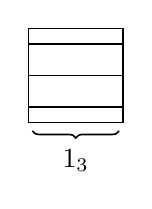
\begin{tikzpicture}[baseline=-0.65ex, scale=0.2]
        \draw[semithick] (-3, -2) to (3, -2);
        \draw[semithick] (-3, 0) to (3, 0);
        \draw[semithick] (-3, 2) to (3, 2);
        \draw (-3, -3) rectangle (3, 3);
        \draw[semithick, decoration={brace,mirror,raise=3pt},decorate]  (-2.75, -3) -- node[below=6pt] {$1_3$} (2.75, -3);
    \end{tikzpicture}
    \quad\quad\quad
    \begin{tikzpicture}[baseline=-0.65ex, scale=0.2]
        \useasboundingbox (-6, -3) rectangle (12, 5);
\begin{knot}[clip width=5, end tolerance=1pt]
        \strand[semithick] (-6, 0) .. controls (-4, 0) and (-5, 2) .. (-3, 2);
        \strand[semithick] (-6, 2) .. controls (-4, 2) and (-5, 0) .. (-3, 0);
        \strand[semithick] (-6, -2) to (-3, -2);
        \strand[semithick] (-3, 0) .. controls (-1, 0) and (-2, -2) .. (0, -2);
        \strand[semithick] (-3, -2) .. controls (-1, -2) and (-2, 0) .. (0, 0);
        \strand[semithick] (-3, 2) to (0, 2);
        \draw (-6, -3) rectangle (0, 3);
        \draw[semithick, decoration={brace,mirror,raise=3pt},decorate]  (-5.75, -3) -- node[below=6pt] {$\beta_1$} (-0.25, -3);
        \strand[semithick] (+6, 0) .. controls (+4, 0) and (+5, 2) .. (+3, 2);
        \strand[semithick] (+6, 2) .. controls (+4, 2) and (+5, 0) .. (+3, 0);
        \strand[semithick] (+6, -2) to (+3, -2);
        \strand[semithick] (+3, 0) .. controls (+1, 0) and (+2, -2) .. (0, -2);
        \strand[semithick] (+3, -2) .. controls (+1, -2) and (+2, 0) .. (0, 0);
        \strand[semithick] (+3, 2) to (0, 2);
        \draw (+6, -3) rectangle (0, 3);
        \strand[semithick] (6+6, 0) .. controls (6+4, 0) and (6+5, 2) .. (6+3, 2);
        \strand[semithick] (6+6, 2) .. controls (6+4, 2) and (6+5, 0) .. (6+3, 0);
        \strand[semithick] (6+6, -2) to (6+3, -2);
        \strand[semithick] (6+3, 0) .. controls (6+1, 0) and (6+2, -2) .. (6+0, -2);
        \strand[semithick] (6+3, -2) .. controls (6+1, -2) and (6+2, 0) .. (6+0, 0);
        \strand[semithick] (6+3, 2) to (6+0, 2);
        \draw (6+6, -3) rectangle (6+0, 3);
        \draw[semithick, decoration={brace,mirror,raise=3pt},decorate]  (0.25, -3) -- node[below=6pt] {$\beta_2\beta_3$} (11.75, -3);
        \draw[semithick, decoration={brace,raise=3pt},decorate]  (6.25, 3) -- node[above=6pt] {$\beta_3$} (11.75, 3);
        \draw[semithick, decoration={brace,raise=3pt},decorate]  (-5.75, 3) -- node[above=6pt] {$\beta_1\beta_2$} (5.75, 3);
    \end{knot}
    \end{tikzpicture}
\]

\begin{proposition}
    Grupa warkoczy jest izomorficzna z~grupę prezentowaną przez generatory $\sigma_1, \ldots, \sigma_{n-1}$ oraz relacje:
    $\sigma_i \sigma_j = \sigma_j \sigma_i$ dla $|i - j| \neq 1$,
    $\sigma_i\sigma_{i+1} \sigma_i = \sigma_{i+1} \sigma_i \sigma_{i+1}$ dla $1 \le i \le n-2$.
\end{proposition}

Generatory $\sigma_i$ posiadają prostą interpretację graficzną:
\[
    \begin{tikzpicture}[baseline=-0.65ex, scale=0.05]
    \useasboundingbox (-15, -10) rectangle (15, 15);
    \begin{knot}[clip width=5, end tolerance=1pt]
        \strand[semithick] (-15, -10) to (-15, 10);
        \strand[semithick] ( 15, -10) to ( 15, 10);
        \strand[semithick] (-5, -10) to (-5, -5) .. controls (-5, 1) and (5, -1) .. (5, 5) to (5, 10);
        \strand[semithick] (-5, 10) to (-5, 5) .. controls (-5, -1) and (5, 1) .. (5, -5) to (5, -10);
        \node  at (-10, 0) {\ldots};
        \node at ( 10, 0) {\ldots};
        \node [above] at (-15, 12) {$1$};
        \node [above] at ( -5, 12) {$i$};
        \node [above] at (  5, 12) {$i+1$};
        \node [above] at ( 15, 12) {$n$};
    \end{knot}
    \end{tikzpicture}
\]

\begin{proposition}
    Grupa warkoczy $B_n$ jest nieprzemienna wtedy i tylko wtedy, gdy $n \ge 3$.
\end{proposition}

\begin{proof}
    Dla $n = 1$ grupa warkoczowa jest trywialna, dla $n = 2$ mamy $B_2 \cong \Z$.

    Jeśli zapomnimy, jak poszczególne pasma krzyżują się, każdy warkocz staje się permutacją zbioru $n$-elementowego.
    To odwzorowanie jest ,,na'' i zgodne ze składaniem warkoczy, dlatego wyznacza homomorfizm $B_n \to S_n$.
    Grupa $S_n$ dla $n \ge 2$ jest nieprzemienna, zatem grupa $B_n$ także taka jest.
\end{proof}

Obrazem generatora $\sigma_i \in B_n$ jest transpozycja $(i, i+1) \in S_n$, co pozwala przepisać prezentację Artina grupy $B_n$ do prezentacji Coxetera grupy symetrii:
\begin{equation}
    S_n = \langle s_1, \ldots, s_{n-1} \mid s_{i}s_{i+1}s_{i} = s_{i+1}s_{i}s_{i+1}, s_i^2 = 1, s_is_j=s_js_i \mbox { dla } |i-j| \ge 2\rangle.
\end{equation}

Jądrem homomorfizmu $B_n \to S_n$ jest podgrupa warkoczy czystych.
Początek i~koniec każdego pasma czystego warkocza znajduje się w tej samej pozycji.

\begin{proposition}
    Jeśli $n \ge 3$, to centrum grupy $B_n$ jest generowane przez warkocz $(\prod_{i = 1}^{n-1} \sigma_i)^n$.
\end{proposition}

\begin{proof}
    Garside w \cite{garside69}.
\end{proof}

Grupa $B_1$ jest trywialna, $B_2$ cykliczna, zaś $B_3$ to grupa podstawowa trójlistnika.
Nie istnieje węzeł, którego grupą podstawową byłaby jednak $B_n$ dla $n \ge 4$: tam elementy $\sigma_1$, $\sigma_n$ oraz generator centrum rozpinają grupę izomorficzną z~$\Z^3$.
Natomiast asferyczna, niezwarta 3-rozmaitość nie może mieć grupy podstawowej $\Z^3$.
Musimy pominąć czysto kohomologiczny dowód faktu, ale zaiste prowadzi to do sprzeczności.

Każdy warkocz można domknąć do węzła, łącząc punkty $(x_i, 1)$ oraz $(x_i, 0)$
łamanymi, których rzuty do płaszczyzny diagramu nie przecinają się.
Jeden węzeł może być przy tym domknięciem różnych warkoczy.
Żaden węzeł nie jest pomijany.
Co ciekawe, domknięcia warkoczy były rozważane przed samymi warkoczami!

\begin{theorem}[Alexander, 1923] \label{alex_thm}
     Każdy splot powstaje przez domknięcie pewnego warkocza.
     \index{twierdzenie!Alexandera}
\end{theorem}

Niech $b \in B_n$ będzie słowem zapisanym na standardowych generatorach.
Oznaczmy przez $b_+$, $b_-$ nieznakowaną sumę dodatnich, ujemnych wykładników.
Jeśli $b_+ - 3b_- \ge n$, to domknięcie warkocza $b$ nie jest achiralne (twierdzenie 5 z~\cite{jones85}).

\begin{theorem}[Markow, 1936]
    % Każdy splot jest domknięciem pewnego warkocza. -- Alexander
    Dwa domknięte warkocze są równoważne jako sploty wtedy i~tylko wtedy,
    gdy jeden powstaje z~drugiego przez ciąg
    sprzężeń: $z_1 \mapsto z_2 z_1 z_2^{-1}$ oraz procesów Markowa,
    które zastępują $n$-warkocz $\beta$ przez $(n+1)$-warkocz $\beta\sigma_n^{\pm 1}$.
\end{theorem}

\begin{proof}
    Kompletny i~godny naśladowania dowód znajduje się w~trudno dostępnej książce \cite{birman74} Birman, więc warto sprawdzić inne materiały:
    Morton opisał w~\cite{mortonhr86} elementarną i~przepiękną ideę ,,nitkowania'',
    Traczyk podał w~\cite{traczyk98} czysto kombinatoryczne, dwuwymiarowe uzasadnienie oparte o~okręgi Seiferta,
    wreszcie jest jeszcze artykuł \cite{birman02} napisany przez Birman i~Menasco.
\end{proof}

\begin{tobedone}
    Introduction to knot theory: Summary of the lecture by Gregor Schaumann 2016 zawiera informację, że dwa diagramy warkoczy przedstawiają ten sam warkocz wtedy i tylko wtedy, gdy można między nimi przechodzić przy użyciu: tożsamości wężowych oraz ruchów Turaeva.
    Brakuje źródła z krótkim dowodem.
    Możliwe, że w "Operator invariants of ..." 1989.
\end{tobedone}

Problem słowa (czy dane słowo przedstawia element neutralny?) oraz sprzężoności (czy dwa słowa są sprzeżone?) są rozwiązalne w~grupach warkoczowych.
Problem, czy dwa słowa prezentują równoważne węzły -- nie.

\index{reprezentacja Burau}
Na zakończenie sekcji wspomnijmy o~macierzowej reprezentacji Burau.
Wyznaczona jest ona przez obrazy generatorów:
\begin{equation}
    \varphi(\sigma_i) = I_{i-1} \oplus \begin{pmatrix}
        1-t & t \\
        1   & 0
    \end{pmatrix} \oplus I_{n-i-1}
\end{equation}
Reprezentacja $\varphi$ jest wierna dla $n = 2, 3$.
Moody pokazał, że reprezentacja nie jest wierna dla $n > 8$, Long, Paton ulepszyli jego podejście i otrzymali mocniejszą nierównosć $n > 5$.
Ich kontrukcja korzysta z~pewnej zamkniętej krzywej na sześciokrotnie przekłutym dysku o~pewnych cechach homologicznych.
Podobnymi metodami Bigelow pokazał u schyłku stulecia \cite{bigelow99}, że jeśli
\begin{align}
    \psi_1 & = \sigma_3^{{-1}}\sigma_2\sigma_1^2\sigma_2\sigma_4^3\sigma_3\sigma_2, \\
\psi_2 & = \sigma_4^{{-1}}\sigma_3\sigma_2\sigma_1^{{-2}}\sigma_2\sigma_1^2\sigma_2^2\sigma_1\sigma_4^5,
\end{align}
to komutator $[\psi_1^{{-1}}\sigma_4\psi_1,\psi_2^{{-1}}\sigma_4\sigma_3\sigma_2\sigma_1^2\sigma_2\sigma_3\sigma_4\psi_2]$ należy do jądra.
Czy reprezentacja Burau dla $B_4$ jest wierna?
Negatywna odpowiedź na to pytanie prawie na pewno prowadziłaby do
nietrywialnego węzła, którego wielomianem HOMFLY jest $1$,
natomiast odpowiedź pozytywna raczej nie ma aż tak dramatycznych następstw.

Grupy $B_n$ mogą być obiektem badań algebry bez związku z~teorią węzłów.

\begin{proposition}
    Grupa warkoczy $B_n$ jest beztorsyjna dla każdego $n \ge 1$.
\end{proposition}

Istnieje wiele dowodów tego faktu: pierwszy korzystał z~krótkich ciągów dokładnych (Fadell, Neuwirth 1965), później podano oparty o~struktury Garside'a (Garside 1969), czysto teoriogrupowy pochodzi od Dyera (1980).
My przedstawimy inne rozumowanie, opisując przy tym ciekawy sam w sobie porządek Dehornoya.

\begin{proof}
    Mówimy, że grupa $G$ jest lewo-porządkowalna, jeśli można wyposażyć ją w~zupełny porządek $<$, niezmienniczy na mnożenie z lewej strony.
    To znaczy, dla każdych $a, b, c \in G$, z~nierówności $a < b$ wynika $ca < cb$.
    Wtedy zbiór $P = \{g \in G \mid e < g\}$ nazywamy półgrupą elementów dodatnich.
    Łatwo widać, że $G$ jest sumą rozłączną $P \sqcup \{e\} \sqcup P^{-1}$.
    Odwrotnie, każde takie rozbicie wyznacza porządek: wystarczy zdefiniować $a < b \iff a^{-1}b \in P$.

    Dehornoy znalazł taki porządek dla grupy warkoczowej $B_n$ w~\cite{dehornoy94}.
    Za zbiór $P$ elementów dodatnich wziął te słowa na standardowych generatorach, które dla pewnego $i$ zawierają $\sigma_i$, ale nie $\sigma_i^{-1}$ ani $\sigma_j^{\pm 1}$ dla $j < i$.
    Pokazanie, że $P$ jest półgrupą nie sprawia trudności, ale tego, że jest dobrze określonym zbiorem stanowi bardzo nietrywialne zadanie.

    Lewo-porządkowalna grupa jest beztorsyjna.
    Istotnie, ustalmy element $g \in G$ różny od elementu neutralnego.
    Bez straty ogólności niech $e < g$, przemnóżmy tę nierówność stronami przez $g$.
    Dostaniemy tak nową nierówność $g < g^2$.
    Powtarzając proces otrzymujemy łańcuch $e < g < g^2 < g^3 < \ldots$.
    Skoro $<$ jest porządkiem, nie jest możliwe by któryś z elementów $g^n$ był neutralny.
\end{proof}

\begin{proposition}
    Grupa warkoczy $B_n$ jest grupą Hopfa dla każdego $n \ge 1$: nie jest izomorficzna z żadnym ze swoich właściwych ilorazów.
\end{proposition}

\begin{proof}
    Podręcznik \cite{magnus66} dobrze wyjaśnia różne idee stojące za dowodem, który podamy.

    Mówimy, że grupa $G$ jest rezydualnie skończona, jeśli przekrój jej podgrup skończonego indeksu jest trywialny.
    Łatwo widać, że własność ta przenosi się na wszystkie podgrupy grupy $G$.
    Baumslag zauważył, że jeśli grupa $G$ jest skończenie generowana i~rezydualnie skończona, to grupa jej automorfizmów $\operatorname{Aut} G$ jest rezydualnie skończona.
    Grupa $G = \Z^2$ spełnia te założenia.
    Wolna grupa $F_2$ jest podgrupą grupy automorfizmów $\Z^2$, na przykład
    \begin{equation}
        F_2 \simeq \left\langle
        \begin{pmatrix}
            1 & 2 \\
            0 & 1
        \end{pmatrix},
        \begin{pmatrix}
            1 & 0 \\
            2 & 1
        \end{pmatrix}
        \right\rangle \subseteq \operatorname{Aut} \Z^2.
    \end{equation}
    Wszystkie grupy wolne $F_n$, $n \in \N$, są podgrupami grupy $F_2$, dlatego także są rezydualnie skończone, a z nimi grupa warkoczy, gdyż $B_n \subseteq \operatorname{Aut} F_n$.

    Malcew pokazał, że skończenie generowana i~rezydualnie skończona grupa jest grupą Hopfa.
    Krótki dowód tego faktu można znaleźć w~sekcji 6.5 książki \cite{magnus66}.
\end{proof}

\subsection{Liczba warkoczowa} % (fold)
\label{sub:braid_number}
\index{liczba!warkoczowa}
Z angielskiego \emph{braid number}.

\begin{definition}
    Liczba warkoczowa to minimalna liczba pasm, na których można zapleść warkocz, którego domknięciem jest wyjściowy splot.
\end{definition}

Tylko jeden węzeł ma liczbę warkoczową $1$, jest to niewęzeł.
Dwuwarkoczowe są dokładnie węzły torusowe typu $(2, n)$ dla $|n| \ge 3$.
Węzły spełniające $\operatorname{br} (K) = 3$ nie zostały jeszcze sklasyfikowane.
Liczba warkoczowa splotu zależy od orientacji ogniw i~trudno wyznacza się w~ogólnym przypadku.

\begin{proposition}
    Węzeł o~$n$ skrzyżowaniach można zapleść na $n - 1$ pasmach.
\end{proposition}

Powyższe ograniczenie ($\operatorname{b} \le \operatorname{cr} - 1$) nie jest zbyt użyteczne, równość mamy jedynie dla trójlistnika i ósemki.
Dokładną wartość liczby warkoczowej znamy między innymi dla węzłów torusowych (fakt \ref{braid-for-forus}).

Wielomian Alexandera wykrywa czasami węzły, których nie otrzyma się przez domykanie ,,małych'' warkoczy.
Przytoczone tu wyniki pochodzą z pracy \cite{jones85} Jonesa, gdzie nie ma jednak ich dowodów.
Jeśli $|\alexander(i)| > 3$, to węzeł nie jest domknięciem 3-warkocza (wniosek 23).
Ta implikacja jest skuteczna przy 43 z 59 węzłów o mniej niż 10 skrzyżowaniach.
Jeśli zaś spełniona jest nierówność $\alexander (\exp (2\pi i / 5)) > 13/2$, nie jest on domknięciem 4-warkocza (wniosek 24).
Prawdopodobnie nie istnieją podobne warunki dla 5-warkoczy.

% Koniec podsekcji Liczba warkoczowa

% Koniec sekcji warkocze